\documentclass{article}
\usepackage[utf8]{inputenc}
\usepackage[english]{babel}
\usepackage{graphicx}
\usepackage{float}
\usepackage{amsmath}

\title{Boltzmann Machine}
\author{Kevin Jacobs, Zhuoran Liu, Ankur Ankan}

\begin{document}
\section{Introduction}
\subsection{Boltzmann Machines}
A Boltzmann Machine consists of a set of binary units, $ s $ and all these units are 
connected to each other with a weight, $ w_{ij} $ associated with each connection.
The global energy, $ E $ of the Boltzmann Machine is given by:

$$ E = - \left(\sum_{i<j} w_{ij} s_i s_j + \sum_{i} \theta_i s_i \right) $$

While learning from data, we try to adjust the weight parameters such that the
stationary distribution of the Boltzmann machine closly represents our dataset.
For determining the stationary distribution of the Boltzmann Machine we start
with random states for all the binary units and iterate over them setting them
to $ +1 $ with a probability of $ \frac {1} {1 + e^{-2a_i}} $, $ -1 $ otherwise.
After a few iterations the machine converges to its stationary distribution.

Now for comparing this stationary distribution to our dataset we generate some
samples from the Boltzmann Machine and using that we compute the free expections
using:

$$ <s_i> = \sum_{s} s_i p(s), \quad <s_i s_j> = \sum_{s} s_i s_j p(s) $$

Similarly we compute clamped expectations from our dataset using:

$$ <s_i>_{c} = \frac{1}{P} \sum_{\mu} s_i^{\mu}, \quad <s_i s_j>_{c} = \frac{1}{P}
\sum_{\mu} s_i^{\mu} s_j^{\mu} $$

and then we update our weights based on these values:

\begin{equation} \begin{split}
& w_{ij} (t+1) = w_{ij}(t) + \eta \frac{\partial L}{\partial w_{ij}} \\
& \theta_i (t+1) = \theta_i (t) + \eta \frac{\partial L}{\partial \theta_i} \\
& \frac{\partial L}{\partial \theta_i} = <s_i>_c - <s_i> \\
& \frac{\partial L}{\partial w_{ij}} = <s_i s_j>_c - <s_i s_j> 
\end{split} \end{equation}

\section{Research Questions}
\begin{enumerate}
  \item Adding noise to the MNIST Dataset
  \item Sampling vs Mean Field
\end{enumerate}

\section{Results}

\subsection{Accuracy of the model with varying levels of noise}
Each image in the MNIST dataset is represented by a 28x28 pixel. We first 
binarized it and added noise so that the matix $ C $ doesn't get singular.

For adding the noise to the image we created a noise mask for each pixel. Each
pixel in the mast has a value of $ -1 $ with probability $ p $ and value $ 1 $
with probability $ 1-p $. Then we do an element-wise multiplication of the 
binary image and the noise mask. Therefore when $ p=0 $, there shouldn't be any
distortion in the image whereas for $ p=1 $ every bit should be flipped but 
there won't be any change in the structure. For $ p=0.5 $, the maximum noise
will be obtained and the image will be completely distorted. We can see these
effects in Fig. \ref{fig:noise_level}.

\begin{figure}[h]
  \centering
  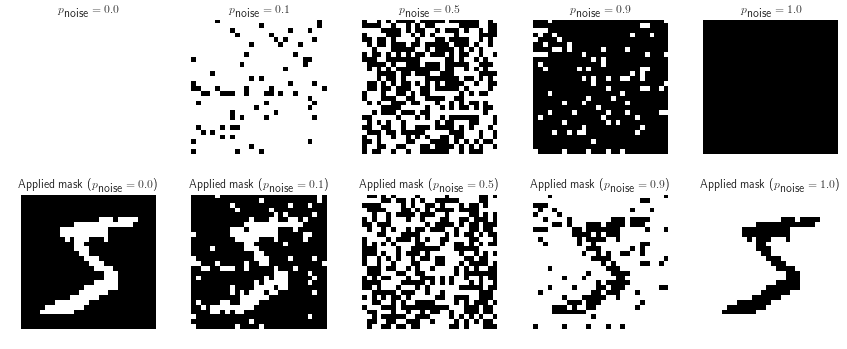
\includegraphics[width=\textwidth]{noise}
  \caption{Different noise levels along with the final masked images}
  \label{fig:noise_level}
\end{figure}

We tried to run our Boltzmann machine on varying levels of noise and computed
the accuracy of our model.

\begin{figure}[h]
  \centering
  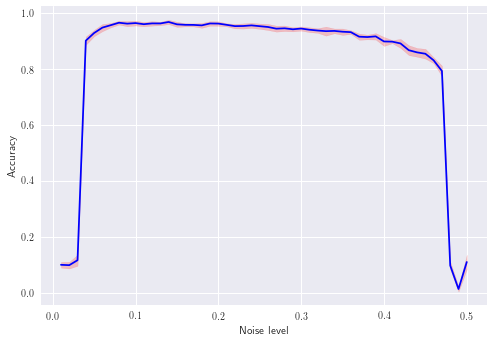
\includegraphics[width=\textwidth]{noise_vs_acc}
  \caption{Accuracy of the model with varying noise level}
  \label{fig:noise_vs_acc}
\end{figure}

There are 3 main features of the graph:
\begin{enumerate}

  \item \textbf {Low accuracy at low noise levels} \break
    In Fig. \ref{fig:noise_vs_acc}, we can see that for very low levels of noise 
    (around 0.00 - 0.03) we have an accuracy of around $ 0.1 $ which is 
    equivalent to random guessing. This low accuracy can be explained by the 
    fact that due to low noise levels some of the pixels in the all the images
    are the same. For example the top-left pixel or the top-right pixel will
    be off in almost all the images. And these constant pixels makes the matrix
    $ C $ approach towards singularity resulting in low accuracy.

  \item \textbf{Highest accuracy at around noise level of 0.1} \break
    The accuracy of the model starts increasing at around $ p=0.04 $, gets 
    around $ 0.9 $ accuracy for $ p \approx 0.5 $ reaching the maximum at 
    $ p \approx 0.1 $ and the gradually decrease as we increase the noise
    level in the data.

  \item \textbf{Dip at $ p=0.47 $ and accuracy of $ 0.1 $ at $ p=0.5 $} \break
    We see a dip in the accuracy value at $ p=0.47 $ where it is almost $ 0 $.
    We coudn't find any good possible explanation for this behaviour. For 
    $ p = 0.5 $ we again get an accuracy of $ 0.1 $. This behaviour can be 
    explained since our images are completely distored now, the model's 
    performace is equivalent to random guessing.

\end{enumerate}

\begin{figure}[ht]
  \centering
  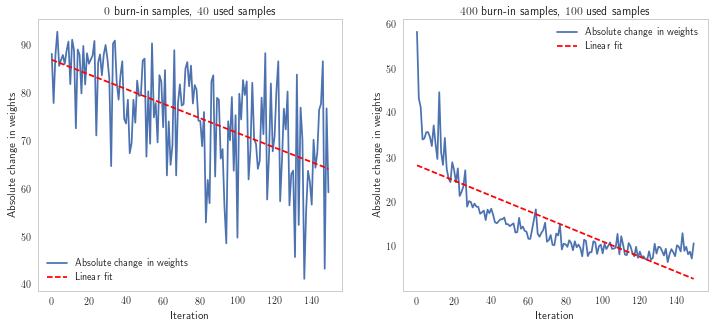
\includegraphics[width=\textwidth]{sampling}
  \caption{Absolute change in weight with iteration}
  \label{fig:sampling}
\end{figure}

\begin{figure}[ht]
  \centering
  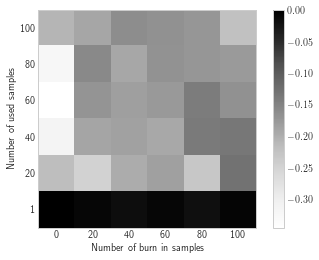
\includegraphics[width=\textwidth]{sampling_grid}
  \caption{Variation of slope for different values of used samples and burn in 
  samples}
  \label{fig:sampling_grid}
\end{figure}

\subsection{Comparision of Sampling Methods and Mean Field Approximation}
For learning a Boltzmann machine we need to compare the free and the clamped
statistics. The probability distribution represented by a Boltzmann machine
is given by:

$$ p(s) = \frac{1}{Z} e^{-E(s)} $$
where: 
\begin{equation}
  \begin{split}
    & E(s) = - \frac{1}{2} \sum_{ij} w_{ij} s_i s_j  + \sum_i \theta_i s_i \\
    & Z = \sum exp(-E(s)) 
  \end{split}
\end{equation}

Here if we try to compute the distribution using any exact method we will need
to compute the value of $ Z $ for which we will need to compute the sum over
all the possible $ 2^n $ states of the Boltzmann machine. This is not feasible 
even in the case of relatively smaller networks because we need to compute the 
free statistics in each iteration until convergence. Therefore we need to use
some approximate techniques. For the assignment we used Gibbs sampling and 
Mean Field theory for approximating the free statistics.

\begin{enumerate}
  \item \textbf{Behaviour in case of Gibbs Sampling}
    We tested the effect of varying the number of samples and burn in period on
    the convergence of our learning rule. For this we used a network of 10 
    neurons and trained on 50 random input patterns. We initialized the weights
    and biases using random samples from a Normal Distribution with mean 0 and 
    variance 1.

    For comparing the rate of convergence, we fitted a straight line to the 
    absolute change in weights with number of iterations as shown in Fig. 
    \ref{fig:sampling}. We also plotted a grid (Fig. \ref{fig:sampling_grid}) for 
    value of slope for different values of burn-in samples and number of used
    samples.


  \item \textbf{Approximating using Mean Field Theory}
    The other approach for approximating the probability distribution is to 
    use Mean Field Theory. As we saw earlier the problem in computing the probability 
    distribution was to compute $ Z $. We can use Mean Field to approximate the
    value of $ Z $. 

\end{enumerate}

\begin{figure}[ht]
  \centering
  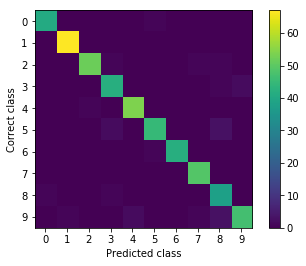
\includegraphics[width=\textwidth]{confusion}
  \caption{Confusion Matrix for classifying all the 10 digits}
  \label{fig:confusion}
\end{figure}

\section{Conclusion}
We were able to get a good accuracy for classification using the Boltzmann 
Machine. The accuracy score using the sampling method was slightly higher than
what we got using the mean field approximation. Our classifier was slightly 
confused in a few cases like between 8 and 5, 3 and 5 as we can see in Fig. 
\ref{fig:confusion}. This happens because the pattern for these digits are 
similar and should be avoidable using some preprocessing steps like rotation
of images. Also as expected the Mean Field Approximation is computationally 
much cheaper than Gibbs Sampling. Training using Mean Field took an average of
1.84 seconds whereas Gibbs sampling took an average of 18.4 sec.

\section{Appendix}

\end{document}
